\section{Specifica della componente model}

Questa componente consente di rappresentare i dati e gestire la loro persistenza, e viene suddivisa in due parti: \textit{client} e \textit{server}. 

\subsection{Client}

Il \textit{model} lato \textit{client} consente di gestire i dati dell'applicazione e la comunicazione con il \textit{server\ped{G}}.

La componente è formata dalle seguenti \textit{classi}:
\begin{itemize}
	\item \hyperref[userDataModel]{\model{}.U\fshyp{}ser\fshyp{}Da\fshyp{}ta\fshyp{}Mo\fshyp{}del};
	\item \hyperref[processModel]{\model{}.Pro\fshyp{}cess\fshyp{}Mo\fshyp{}del};
	\item \hyperref[processDataModel]{\model{}.Pro\fshyp{}cess\fshyp{}Da\fshyp{}ta\fshyp{}Mo\fshyp{}del};
	\item \hyperref[stepModel]{\model{}.Step\fshyp{}Mo\fshyp{}del};
	\item \hyperref[processCollection]{\collection{}.Pro\fshyp{}cess\fshyp{}Col\fshyp{}lec\fshyp{}tion};
	\item \hyperref[processDataCollection]{\model{}.Pro\fshyp{}cess\fshyp{}Da\fshyp{}ta\fshyp{}Col\fshyp{}lec\fshyp{}tion};
	\item \hyperref[stepCollection]{\collection{}.Step\fshyp{}Col\fshyp{}lec\fshyp{}tion}.
\end{itemize}

\subsubsection{Package \model{}}

\paragraph{UserModel}
\label{userDataModel}

\begin{figure}[H] \centering 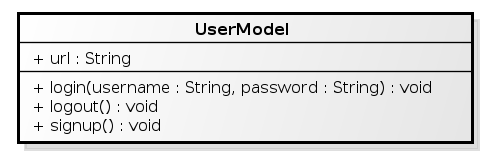
\includegraphics[width=%
\textwidth]
{./classi/client/model/UserModel.png} \caption{Diagramma classe  \textit{UserModel}}
\end{figure}

\begin{flushleft}
\begin{itemize}
\item \textbf{Descrizione:} Classe che permette di gestire i dati di una sessione di un utente autenticato o di un \textit{Process Owner\ped{G}};
\item \textbf{Attributi:}
\begin{sloppypar}
\begin{itemize}
\item \texttt{+ String url:}\\ campo dati di ridefinito da \texttt{Backbone.Model} che contiene l'indirizzo \textit{url\ped{G}} per comunicare con il \textit{server\ped{G}};
\end{itemize}
\end{sloppypar}
\item \textbf{Metodi:}
\begin{sloppypar}
\begin{itemize}
\item \texttt{+ void login(String username, String password):}\\ delega al server il controllo delle credenzili e, al completamento della richiesta, salva i dati di sessione in caso di successo;
\item \texttt{+ void logout():}\\ cancella di dati di sessione dell'utente;
\item \texttt{+ void signup():}\\ effettua una richiesta di registrazione al \textit{server\ped{G}} inviando i dati della classe.
\end{itemize}
\end{sloppypar}
\end{itemize}
\end{flushleft}

\paragraph{ProcessModel}
\label{processModel}

\begin{figure}[H] \centering 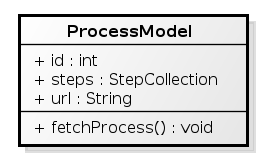
\includegraphics[width=%
\textwidth]
{./classi/client/model/ProcessModel.png} \caption{Diagramma classe  \textit{ProcessModel}}
\end{figure}

\begin{flushleft}
\begin{itemize}
\item \textbf{Descrizione:} Classe che permette di gestire i dati di un processo, e di salvarli o recuperarli dal \textit{server\ped{G}};
\item \textbf{Relazioni con altri componenti:}
\begin{sloppypar}
La classe contiene un oggetto di tipo \texttt{\collection{}.Step\fshyp{}Col\fshyp{}lec\fshyp{}tion}.
\end{sloppypar}
\item \textbf{Attributi:}
\begin{sloppypar}
\begin{itemize}
\item \texttt{+ int id:}\\ campo dati ridefinito da \texttt{Backbone.model} che rappresenta l'identificatore del processo;
\item \texttt{+ StepCollection steps:}\\ campo dati di tipo \texttt{\collection{}.Step\fshyp{}Col\fshyp{}lec\fshyp{}tion} che contiene la collezione dei passi del processo;
\item \texttt{+ String url:}\\ campo dati di ridefinito da \texttt{Backbone.Model} che contiene l'indirizzo \textit{url\ped{G}} per comunicare con il \textit{server\ped{G}};
\end{itemize}
\end{sloppypar}
\item \textbf{Metodi:}
\begin{sloppypar}
\begin{itemize}
\item \texttt{+ void fetchProcess():}\\ recupera dal \textit{server\ped{G}} i dati del processo, e i dati dei passi che assegna alla collezione \texttt{steps}, sincronizzando le operazioni.
\end{itemize}
\end{sloppypar}
\end{itemize}
\end{flushleft}

\paragraph{ProcessDataModel}
\label{processDataModel}

\begin{figure}[H] \centering 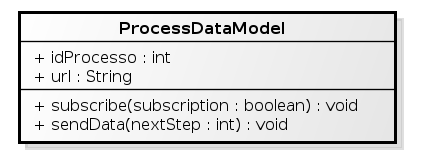
\includegraphics[width=%
\textwidth]
{./classi/client/model/ProcessDataModel.png} \caption{Diagramma classe  \textit{ProcessDataModel}}
\end{figure}

\begin{flushleft}
\begin{itemize}
\item \textbf{Descrizione:} Classe che permette di gestire i dati inviati da un utente relativi ad un processo, e di salvarli o recuperarli dal \textit{server\ped{G}};
\item \textbf{Attributi:}
\begin{sloppypar}
\begin{itemize}
\item \texttt{+ int idProcesso:}\\ rappresenta l'identificatore del processo a cui i dati si riferiscono;
\item \texttt{+ String url:}\\ campo dati di ridefinito da \texttt{Backbone.Model} che contiene l'indirizzo \textit{url\ped{G}} per comunicare con il \textit{server\ped{G}};
\end{itemize}
\end{sloppypar}
\item \textbf{Metodi:}
\begin{sloppypar}
\begin{itemize}
\item \texttt{+ void subscribe(bool subscription):}\\ effettua una richiesta di iscrizione o disiscrizione al \textit{server\ped{G}} a seconda del valore del parametro \textit{subscription}, riguardante il processo con "id" \texttt{idProcesso};
\item \texttt{+ void sendData(int nextStep):}\\ invia al \textit{server\ped{G}} i dati della classe e l'id del prossimo passo da eseguire, che identifica una condizione del processo con "id" \texttt{idProcesso}.
\end{itemize}
\end{sloppypar}
\end{itemize}
\end{flushleft}

\paragraph{StepModel}
\label{stepModel}

\begin{figure}[H] \centering 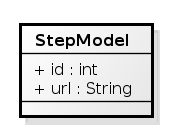
\includegraphics[width=%
\textwidth]
{./classi/client/model/StepModel.png} \caption{Diagramma classe  \textit{StepModel}}
\end{figure}

\begin{flushleft}
\begin{itemize}
\item \textbf{Descrizione:} Classe che permette di gestire i dati di un passo di un processo, e di salvarli o recuperarli dal \textit{server\ped{G}};
\item \textbf{Attributi:}
\begin{sloppypar}
\begin{itemize}
\item \texttt{+ int id:}\\ campo dati ridefinito da \texttt{Backbone.model} che rappresenta l'identificatore del passo;
\item \texttt{+ String url:}\\ campo dati di ridefinito da \texttt{Backbone.Model} che contiene l'indirizzo \textit{url\ped{G}} per comunicare con il \textit{server\ped{G}};
\end{itemize}
\end{sloppypar}
\end{itemize}
\end{flushleft}

\subsubsection{Package \collection{}}

\paragraph{ProcessCollection}
\label{processCollection}

\begin{figure}[H] \centering 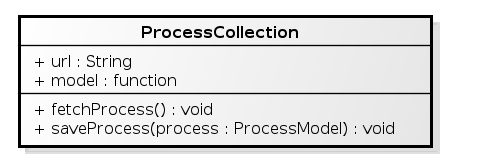
\includegraphics[width=%
\textwidth]
{./classi/client/model/ProcessCollection.png} \caption{Diagramma classe  \textit{ProcessCollection}}
\end{figure}

\begin{flushleft}
\begin{itemize}
\item \textbf{Descrizione:} Classe che permette di gestire un insieme di dati inviati da un utente relativi ad un processo;
\item \textbf{Relazioni con altri componenti:}
\begin{sloppypar}
La classe definisce una collezione di \texttt{\model{}.Process\fshyp{}Da\fshyp{}ta\fshyp{}Mo\fshyp{}del}.
\end{sloppypar}
\item \textbf{Attributi:}
\begin{sloppypar}
\begin{itemize}
\item \texttt{+ String url:}\\ campo dati di ridefinito da \texttt{Backbone.Collection} che contiene l'indirizzo \textit{url\ped{G}} per comunicare con il \textit{server\ped{G}};
\item \texttt{+ function model:}\\ campo dati di ridefinito da \texttt{Backbone.Collection} che contiene la definizione della classe \texttt{\model{}.Process\fshyp{}Da\fshyp{}ta\fshyp{}Mo\fshyp{}del};
\end{itemize}
\end{sloppypar}
\item \textbf{Metodi:}
\begin{sloppypar}
\begin{itemize}
\item \texttt{+ void fetchProcesses():}\\ richiede al server la lista dei processi a cui l'utente identificato dai dati di sessione può accedere;
\item \texttt{+ void saveProcess(ProcessModel process):}\\ aggiunge il processo \texttt{process} alla collezione dei processi nel \textit{serve\ped{G}}.
\end{itemize}
\end{sloppypar}
\end{itemize}
\end{flushleft}

\paragraph{ProcessDataCollection}
\label{processDataCollection}

\begin{figure}[H] \centering 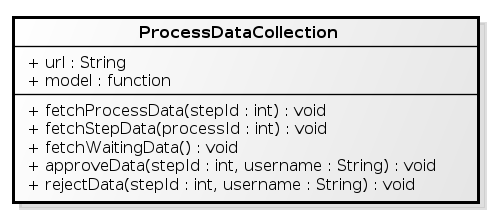
\includegraphics[width=%
\textwidth]
{./classi/client/model/ProcessDataCollection.png} \caption{Diagramma classe  \textit{ProcessDataCollection}}
\end{figure}

\begin{flushleft}
\begin{itemize}
\item \textbf{Descrizione:} Classe che permette di gestire un insieme di dati inviati dagli utenti;
\item \textbf{Relazioni con altri componenti:}
\begin{sloppypar}
La classe definisce una collezione di \texttt{\model{}.Process\fshyp{}Da\fshyp{}ta\fshyp{}Mo\fshyp{}del}.
\end{sloppypar}
\item \textbf{Attributi:}
\begin{sloppypar}
\begin{itemize}
\item \texttt{+ String url:}\\ campo dati di ridefinito da \texttt{Backbone.Collection} che contiene l'indirizzo \textit{url\ped{G}} per comunicare con il \textit{server\ped{G}};
\item \texttt{+ function model:}\\ campo dati di ridefinito da \texttt{Backbone.Collection} che contiene la definizione della classe \texttt{\model{}.Process\fshyp{}Da\fshyp{}ta\fshyp{}Mo\fshyp{}del};
\end{itemize}
\end{sloppypar}
\item \textbf{Metodi:}
\begin{sloppypar}
\begin{itemize}
\item \texttt{+ void fetchProcessData(int stepId):}\\ richiede al \textit{server\ped{G}} la lista dei dati inviati riguardanti il passo con "id" \texttt{stepId}, ai quali l'utente identificato dai dati di sessione può accedere;
\item \texttt{+ void fetchStepData(int processId):}\\ richiede al \textit{server\ped{G}} la lista dei dati inviati riguardanti il processo con "id" \texttt{processId}, ai quali l'utente identificato dai dati di sessione può accedere;
\item \texttt{+ void fetchWaitingData():}\\ richiede al \textit{server\ped{G}} la lista dei dati inviati che richiedono controllo umano;
\item \texttt{+ void approveData(int stepId, String username):}\\ invia al \textit{server\ped{G}} la richiesta di approvazione dei dati riguardanti il passo con "id" \texttt{stepId} e l'utente con username \texttt{username}.
\item \texttt{+ void rejectData(int stepId, String username):}\\ invia al \textit{server\ped{G}} l'esito negativo del controllo dei dati riguardanti il passo con "id" \texttt{stepId} e l'utente con username \texttt{username}.
\end{itemize}
\end{sloppypar}
\end{itemize}
\end{flushleft}

\paragraph{StepCollection}
\label{stepCollection}

\begin{figure}[H] \centering 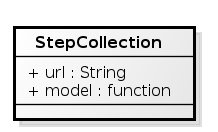
\includegraphics[width=%
\textwidth]
{./classi/client/model/StepCollection.png} \caption{Diagramma classe  \textit{StepCollection}}
\end{figure}

\begin{flushleft}
\begin{itemize}
\item \textbf{Descrizione:} Classe che permette di gestire un insieme di passi di un processo;
\item \textbf{Relazioni con altri componenti:}
\begin{sloppypar}
La classe definisce una collezione di \texttt{\model{}.Step\fshyp{}Mo\fshyp{}del}.
\end{sloppypar}
\item \textbf{Attributi:}
\begin{sloppypar}
\begin{itemize}
\item \texttt{+ String url:}\\ campo dati di ridefinito da \texttt{Backbone.Collection} che contiene l'indirizzo \textit{url\ped{G}} per comunicare con il \textit{server\ped{G}};
\item \texttt{+ function model:}\\ campo dati di ridefinito da \texttt{Backbone.Collection} che contiene la definizione della classe \texttt{\model{}.Step\fshyp{}Mo\fshyp{}del};
\end{itemize}
\end{sloppypar}
\end{itemize}
\end{flushleft}